\chapter{जीव विज्ञान में कृत्रिम बुद्धिमत्ता}
\label{ch:biology}

\lakshyaheading
\begin{itemize}[leftmargin=1.4em]
  \item जीवन की जानकारी को \emph{डेटा} के रूप में समझना - विशेषकर DNA एवं प्रोटीन।
  \item प्रोटीन-संरचना (protein structure) के पूर्वानुमान में AI (AlphaFold)।
  \item चिकित्सा-चित्रों (medical images) में रोग-पहचान हेतु \term{चित्र-वर्गीकरण}{image
        classification}।
  \item प्रजाति-पहचान (species identification) एवं जैव-विविधता में AI।
  \item मुफ़्त उपकरणों एवं सरल Python से जैविक डेटा पर स्वयं प्रयोग।
\end{itemize}

\section{जीवन का डेटा: DNA}

हमारे शरीर की लगभग सम्पूर्ण जानकारी DNA में, केवल चार ``अक्षरों'' - A, T, G, C
(\term{क्षारक}{bases}) - के क्रम में लिखी होती है। मनुष्य के DNA में ऐसे लगभग
3 अरब (3 billion) अक्षर होते हैं। यह इतना विशाल \term{डेटा}{data} है कि इसका विश्लेषण
AI के बिना लगभग असम्भव है।

इन अक्षरों के क्रम (sequence) में ही यह छिपा होता है कि कौन-सा प्रोटीन बनेगा और कोशिका
कैसे कार्य करेगी। AI इन क्रमों में पैटर्न खोजकर बता सकती है कि कोई विशेष क्रम किसी रोग
से जुड़ा है या नहीं - इसी क्षेत्र को \term{जैव-सूचना विज्ञान}{Bioinformatics} कहते हैं।
DNA की द्विकुंडलिनी (double helix) संरचना चित्र~\ref{fig:dna} में दिखाई गई है।

\begin{figure}[h]
\centering
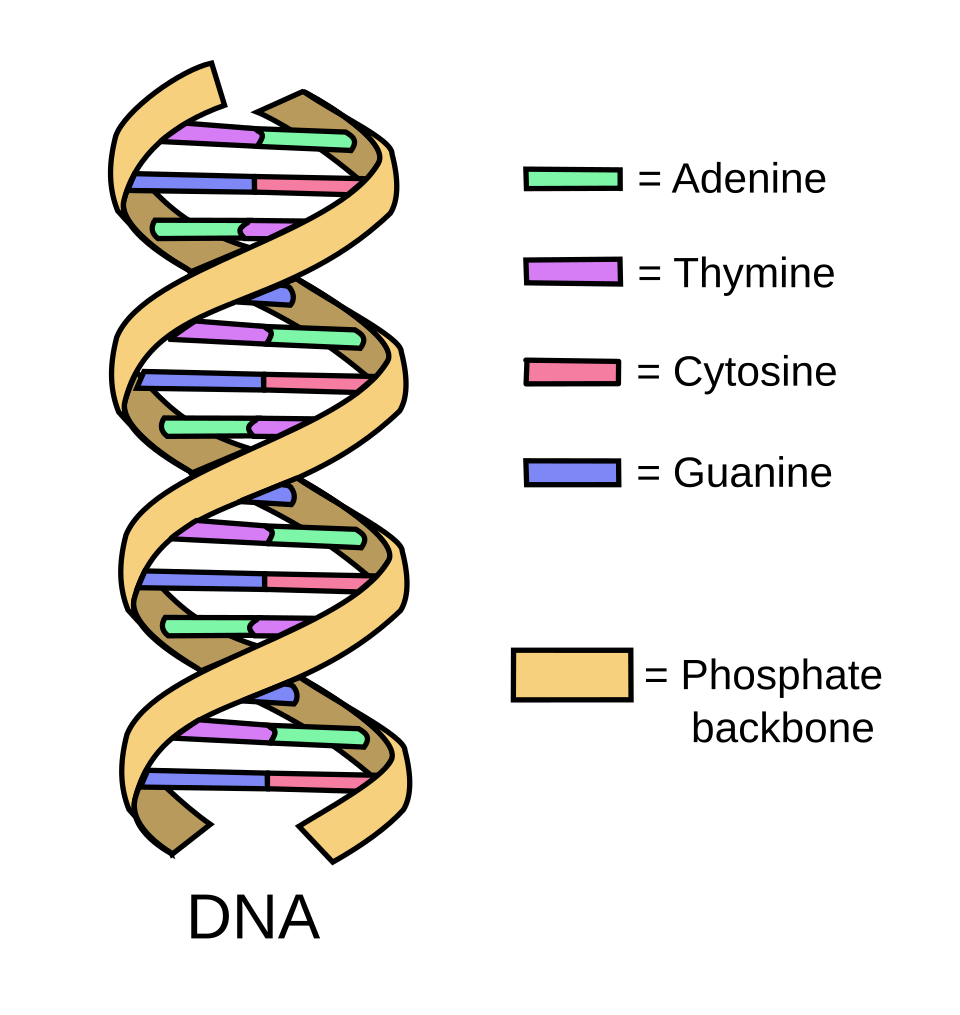
\includegraphics[height=5.2cm]{images/dna.png}
\caption[DNA की द्विकुंडलिनी (double helix)]{DNA की द्विकुंडलिनी (double helix) -- A, T,
G, C क्षारकों का क्रम ही जीवन का विशाल ``डेटा'' है, जिसे AI पढ़ती एवं विश्लेषित करती
है।\imgsrc{Forluvoft, Wikimedia Commons (Public Domain)}}
\label{fig:dna}
\end{figure}

\begin{jante}
मानव जीनोम (human genome) को पूरा पढ़ने वाली ``Human Genome Project'' परियोजना (2003)
में लगभग 13 वर्ष लगे थे। आज वही कार्य उन्नत मशीनों एवं AI की सहायता से कुछ ही घंटों में
सम्भव है।
\end{jante}

\section{प्रोटीन की संरचना: AlphaFold}

प्रोटीन (protein) अमीनो अम्लों (amino acids) की एक लम्बी शृंखला से बनते हैं, परन्तु उनका
कार्य उनकी \emph{त्रि-आयामी (3D) मुड़ी हुई संरचना} पर निर्भर करता है। किसी क्रम से उसकी
3D संरचना का पूर्वानुमान करना दशकों तक जीव विज्ञान की सबसे कठिन समस्याओं में से एक था,
जिसे \term{प्रोटीन-वलन समस्या}{Protein Folding Problem} कहते हैं।

सन् 2021 में DeepMind के \emph{AlphaFold} नामक AI ने इस समस्या को हल करने में ऐतिहासिक
सफलता पाई, और 2022 तक लगभग सभी ज्ञात प्रोटीनों (लगभग 20 करोड़) की 3D संरचना का सटीक
पूर्वानुमान कर दिया। यह AI की सहायता से विज्ञान की एक ऐतिहासिक उपलब्धि
मानी जाती है, क्योंकि इससे नई दवाओं एवं एंज़ाइमों (enzymes) की खोज बहुत तेज़ हो गई।
मूल विचार चित्र~\ref{fig:alphafold} में दर्शाया गया है: एक अमीनो-अम्ल क्रम (input) से
AI सीधे प्रोटीन की 3D संरचना (output) का पूर्वानुमान कर देती है।

\begin{figure}[h]
\centering
\begin{tikzpicture}[font=\sffamily\small, node distance=10mm,
    box/.style={draw=aiblue, thick, fill=ailite, rounded corners,
      minimum height=1.5cm, text width=3cm, align=center, inner sep=4pt},
    ai/.style={draw=aigreen, very thick, fill=aigreenL, rounded corners,
      minimum height=1.5cm, text width=2.6cm, align=center},
    arr/.style={-{Stealth[length=3mm]}, very thick, aigrey}]
  \node[box] (seq) {\footnotesize अमीनो-अम्ल क्रम\\\ttfamily\scriptsize M-K-T-A-Y-\dots};
  \node[ai, right=of seq] (af) {\bfseries AI\\\footnotesize (AlphaFold)};
  \node[box, right=of af] (str) {\footnotesize 3D प्रोटीन संरचना\\\footnotesize (folded structure)};
  \draw[arr] (seq) -- (af) node[midway, above, aigrey, font=\scriptsize] {input};
  \draw[arr] (af) -- (str) node[midway, above, aigrey, font=\scriptsize] {output};
\end{tikzpicture}
\caption{AlphaFold का मूल विचार: क्रम (sequence) से सीधे प्रोटीन की 3D संरचना का
पूर्वानुमान।}
\label{fig:alphafold}
\end{figure}

\begin{sochiye}
एक ही अमीनो-अम्ल क्रम सदैव एक ही आकार में मुड़ता है। इसका अर्थ है कि ``क्रम'' में ही
``आकार'' की जानकारी छिपी है। यह विचार Machine Learning के ``input से output का
पूर्वानुमान'' से किस प्रकार मिलता-जुलता है? चर्चा कीजिए।
\end{sochiye}

\begin{figure}[h]
\centering
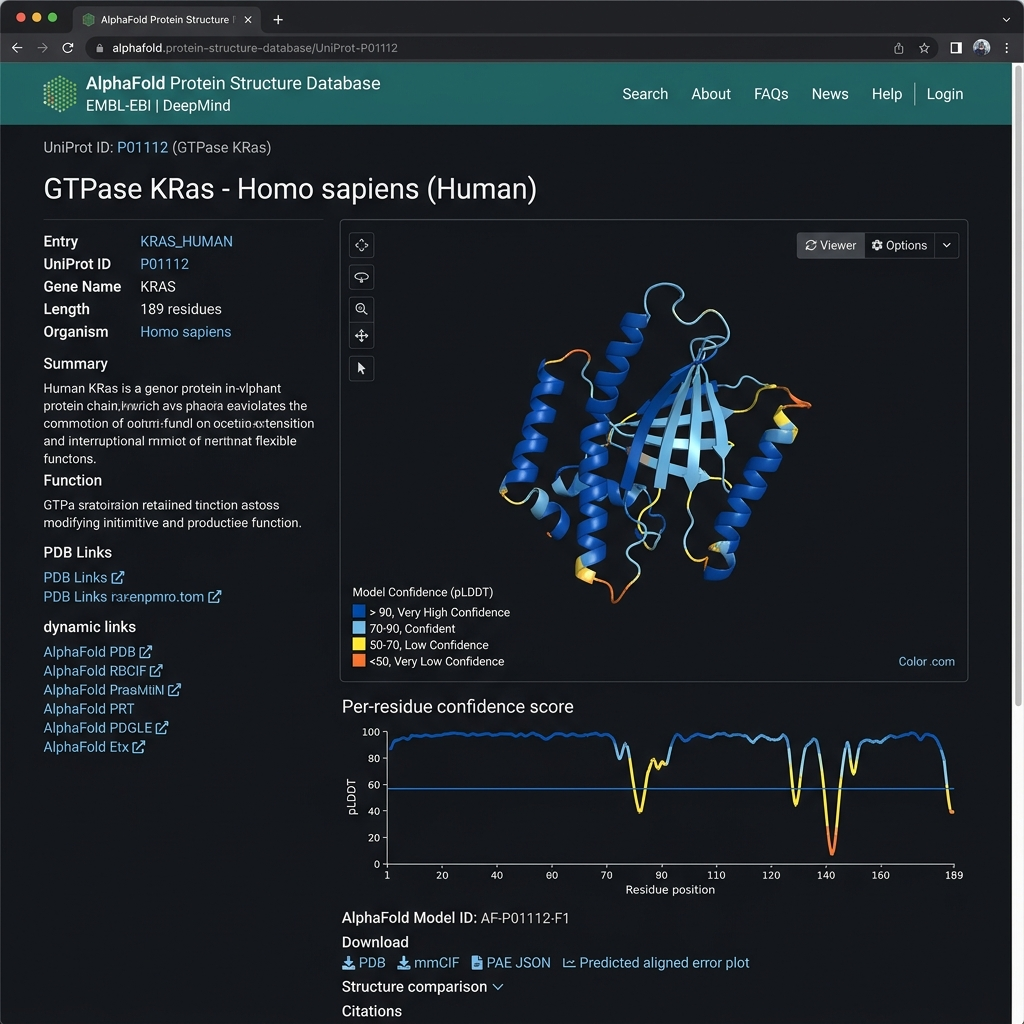
\includegraphics[width=0.82\linewidth]{images/alphafold_db_ui.jpg}
\caption[अल्फाफोल्ड प्रोटीन संरचना डेटाबेस]{अल्फाफोल्ड डेटाबेस (AlphaFold DB) का इंटरफ़ेस -- जहाँ मानव के KRas प्रोटीन (GTPase KRas) की 3D मुड़ी हुई संरचना और उसका स्थान-वार विश्वसनीयता ग्राफ़ (pLDDT score) दर्शाया गया है।}
\label{fig:alphafold-db-ui}
\end{figure}

\section{रोग-निदान में चित्र-पहचान}

जीव विज्ञान एवं चिकित्सा में बहुत-सी जानकारी \emph{चित्रों} के रूप में होती है - जैसे
X-ray, MRI, CT scan, या सूक्ष्मदर्शी (microscope) से ली गई कोशिकाओं की छवियाँ। AI इन
चित्रों में रोग के सूक्ष्म चिह्न पहचान सकती है, जिन्हें कभी-कभी आँख से देखना कठिन होता है।

\begin{itemize}[leftmargin=1.4em]
  \item \textbf{कैंसर-पहचान:} ऊतक (tissue) की छवियों में असामान्य कोशिकाएँ ढूँढना।
  \item \textbf{नेत्र-रोग:} रेटिना (retina) की तस्वीर से मधुमेह-जनित रोग पहचानना।
  \item \textbf{रक्त-जाँच:} सूक्ष्मदर्शी छवि में विभिन्न रक्त-कोशिकाओं की गिनती।
\end{itemize}

\noindent यहाँ ध्यान देने योग्य बात यह है कि AI डॉक्टर का \emph{स्थान} नहीं लेती; वह एक
\term{द्वितीय राय}{second opinion} देती है। अंतिम निर्णय सदैव चिकित्सक ही लेता है।

\begin{jante}
\textbf{भारतीय स्टार्टअप: रोग निदान में क्रांति (Indian Healthcare AI Startups):}
भारत में कई स्वास्थ्य-तकनीक (health-tech) कंपनियाँ चिकित्सा में AI के नवोन्मेषी अनुप्रयोग कर रही हैं। उदाहरण के लिए:
\begin{itemize}[leftmargin=1.2em]
  \item \textbf{Niramai:} यह बेंगलुरु आधारित कंपनी कृत्रिम बुद्धिमत्ता और थर्मल इमेजिंग (Thermal Imaging) का उपयोग करके बिना किसी दर्द या विकिरण (radiation) के बहुत ही प्रारंभिक चरण में स्तन कैंसर (Breast Cancer) की स्क्रीनिंग करती है।
  \item \textbf{Qure.ai:} यह मुंबई आधारित कंपनी AI का उपयोग करके चेस्ट एक्स-रे (Chest X-ray) और सीटी स्कैन का सेकंडों में विश्लेषण कर लेती है। इसका उपयोग सुदूर ग्रामीण क्षेत्रों में तपेदिक (Tuberculosis) और मस्तिष्क आघात (Brain Stroke) की तुरंत पहचान के लिए किया जा रहा है।
\end{itemize}
\end{jante}

\begin{gatividhi}[पत्तियों का वर्गीकरण - image classification]
\textbf{लक्ष्य:} यह अनुभव करना कि मशीन छवियों से प्रजातियाँ कैसे पहचानती है।\\[4pt]
\textbf{सामग्री:} कंप्यूटर/मोबाइल, वेबकैम, इंटरनेट।\\[4pt]
\textbf{चरण:}
\begin{enumerate}[leftmargin=1.6em]
  \item विद्यालय परिसर से 3 भिन्न पौधों की पत्तियाँ एकत्र करें।
  \item \emph{Teachable Machine} में तीन class बनाकर प्रत्येक पत्ती के 20-25 चित्र लें।
  \item मॉडल ``Train'' करें, फिर एक नई पत्ती दिखाकर परिणाम देखें।
  \item बताएँ - किन पत्तियों में मशीन सबसे अधिक भ्रमित (confused) हुई और क्यों?
\end{enumerate}
\textbf{अवलोकन:} समान दिखने वाली पत्तियों में मशीन की सटीकता (accuracy) घट जाती है -
ठीक वैसे ही जैसे मनुष्य भी भ्रमित हो सकता है।
\end{gatividhi}

\section{जैविक डेटा पर Python (एक झलक)}

DNA केवल अक्षरों की एक पंक्ति है, अतः कंप्यूटर उसे आसानी से पढ़ सकता है। नीचे का छोटा
Python कोड किसी DNA क्रम में चारों क्षारकों की गिनती करता है - यह \emph{Bioinformatics}
का सबसे आधारभूत कार्य है। (इसे चलाना अध्याय~5 में सीखेंगे।)

\begin{lstlisting}
# a short DNA sequence
dna = "ATGCGGATTACGCTAGCATGGC"

for base in "ATGC":
    print(base, "count =", dna.count(base))

# GC content - linked to several biological properties
gc = (dna.count("G") + dna.count("C")) / len(dna) * 100
print("GC content =", round(gc, 1), "%")
\end{lstlisting}
\colabnb{https://colab.research.google.com/github/kkreboot/ai-in-science-hindi/blob/main/notebooks/ch4-dna.ipynb}

\noindent यहाँ मशीन कोई जीव विज्ञान नहीं ``जानती''; वह केवल अक्षरों की गिनती कर रही है।
फिर भी यही सरल गिनती किसी जीन की पहचान में पहला कदम बन सकती है।

\section{प्रजाति-पहचान एवं जैव-विविधता}

AI अब क्षेत्र-जीव विज्ञान (field biology) में भी उपयोगी है। मोबाइल ऐप किसी पौधे, पक्षी
या कीट की तस्वीर से उसकी प्रजाति (species) पहचान सकते हैं। इससे विद्यार्थी एवं नागरिक
भी \term{नागरिक विज्ञान}{Citizen Science} में भाग ले सकते हैं और जैव-विविधता
(biodiversity) का डेटा एकत्र कर सकते हैं।

\begin{jante}
\emph{iNaturalist} एवं इसी प्रकार के ऐप करोड़ों तस्वीरों पर प्रशिक्षित हैं। जब आप कोई
तस्वीर डालते हैं, तो AI तुरंत सम्भावित प्रजातियों के नाम सुझा देती है - और यह डेटा
वैज्ञानिकों को प्रजातियों के फैलाव (distribution) का अध्ययन करने में मदद करता है।
\end{jante}

% ---------------- परियोजना ----------------
\begin{pariyojana}[स्थानीय जैव-विविधता का मानचित्र]
\textbf{उद्देश्य:} AI-आधारित प्रजाति-पहचान का उपयोग कर अपने क्षेत्र का जैव-विविधता
डेटा एकत्र करना और उसकी सीमाएँ समझना।\\[4pt]
\textbf{सामग्री:} मोबाइल कैमरा, \emph{iNaturalist} या ``Google Lens'' जैसा ऐप।\\[4pt]
\textbf{कार्य (समूह में, 3-4 विद्यार्थी):}
\begin{enumerate}[leftmargin=1.6em]
  \item दो सप्ताह तक अपने आस-पास के 15-20 पौधों/पक्षियों/कीटों की तस्वीरें लें।
  \item प्रत्येक के लिए ऐप द्वारा सुझाई गई प्रजाति नोट करें।
  \item जाँचें - किन मामलों में AI निश्चित (confident) थी और किनमें संदेह में?
        जहाँ सम्भव हो, किसी पुस्तक या शिक्षक से उत्तर सत्यापित करें।
  \item एक सरल तालिका/मानचित्र बनाएँ जिसमें प्रजाति, स्थान एवं AI की शुद्धता दर्शाई हो।
  \item निष्कर्ष लिखें - स्थानीय डेटा की कमी मॉडल की सटीकता को कैसे प्रभावित करती है?
\end{enumerate}
\textbf{मूल्यांकन:} एकत्र डेटा की विविधता, सत्यापन की गंभीरता एवं निष्कर्ष की
स्पष्टता के आधार पर।
\end{pariyojana}

% ---------------- सारांश ----------------
\section*{सारांश (Summary)}
\addcontentsline{toc}{section}{सारांश}
\begin{itemize}[leftmargin=1.4em]
  \item जीवन की जानकारी DNA में चार क्षारकों (A, T, G, C) के क्रम के रूप में एक विशाल
        डेटा है, जिसका विश्लेषण Bioinformatics में AI द्वारा होता है।
  \item AlphaFold ने प्रोटीन-वलन (protein folding) की दशकों पुरानी समस्या को AI से
        हल करने में बड़ी सफलता पाई।
  \item चिकित्सा-चित्रों में रोग-पहचान image classification का महत्वपूर्ण उपयोग है,
        जहाँ AI द्वितीय राय देती है पर निर्णय चिकित्सक का होता है।
  \item प्रजाति-पहचान ऐप नागरिक विज्ञान एवं जैव-विविधता अध्ययन को सरल बनाते हैं।
  \item DNA जैसे डेटा पर सरल Python से ही जैविक विश्लेषण आरम्भ किया जा सकता है।
\end{itemize}

% ---------------- अभ्यास ----------------
\section*{अभ्यास (Exercises)}
\addcontentsline{toc}{section}{अभ्यास}
\textbf{अ. रिक्त स्थान भरिए:}
\begin{enumerate}[leftmargin=1.6em]
  \item DNA चार क्षारकों \rule{2.8cm}{0.4pt} के क्रम से बनता है।
  \item प्रोटीन की 3D संरचना के पूर्वानुमान करने वाली प्रसिद्ध AI का नाम
        \rule{2.8cm}{0.4pt} है।
  \item जैविक डेटा के विश्लेषण के क्षेत्र को \rule{2.8cm}{0.4pt} कहते हैं।
\end{enumerate}

\textbf{ब. लघु उत्तरीय:}
\begin{enumerate}[leftmargin=1.6em]
  \item ``DNA एक डेटा है'' - इस कथन को समझाइए।
  \item चिकित्सा में AI ``डॉक्टर का स्थान नहीं लेती'' - इसका क्या अर्थ है?
  \item AlphaFold की उपलब्धि जीव विज्ञान के लिए क्यों महत्वपूर्ण है?
\end{enumerate}

\textbf{स. क्रियात्मक / दीर्घ उत्तरीय:}
\begin{enumerate}[leftmargin=1.6em]
  \item पत्तियों के वर्गीकरण वाली गतिविधि कीजिए तथा यह लिखिए कि चित्रों की संख्या
        बढ़ाने पर सटीकता पर क्या प्रभाव पड़ा।
  \item दिए गए DNA क्रम \texttt{ATGCATGC} में प्रत्येक क्षारक की गिनती कीजिए तथा
        GC content ज्ञात कीजिए।
  \item ``नागरिक विज्ञान में AI की भूमिका'' पर एक संक्षिप्त निबंध लिखिए।
\end{enumerate}

\begin{mcq}
  \item DNA में कितने प्रकार के क्षारक (bases) होते हैं?
    \begin{choices}\item 2 \item 3 \item 4 \item 5\end{choices}
  \item प्रोटीन की 3D संरचना का पूर्वानुमान करने वाला प्रसिद्ध AI तंत्र है:
    \begin{choices}\item AlphaFold \item AlphaGo \item DeepFace \item ChatGPT\end{choices}
  \item DNA क्रमों में पैटर्न खोजने वाला क्षेत्र कहलाता है:
    \begin{choices}\item जैव-सूचना विज्ञान (Bioinformatics) \item ज्योतिष
      \item भू-विज्ञान \item क्रिस्टलोग्राफी\end{choices}
  \item चिकित्सा-छवियों में रोग पहचानने में AI की भूमिका है:
    \begin{choices}\item डॉक्टर का स्थान लेना \item द्वितीय राय (second opinion) देना
      \item दवा बनाना \item शल्यक्रिया करना\end{choices}
\end{mcq}

\begin{mukhyashabd}
\textbf{क्षारक (bases: A,T,G,C)}, \textbf{जैव-सूचना विज्ञान (Bioinformatics)},
\textbf{प्रोटीन-वलन समस्या}, \textbf{AlphaFold}, \textbf{चित्र-वर्गीकरण (image classification)},
\textbf{द्वितीय राय (second opinion)}, \textbf{नागरिक विज्ञान (Citizen Science)},
\textbf{GC content}।
\end{mukhyashabd}
\selfcheckqr{https://forms.gle/aivigyan-ch4-quiz}
